\documentclass[basic]{inVerba-notes}

\newcommand{\userName}{Cullyn Newman}
\newcommand{\class}{BI:\@ 428}
\newcommand{\theTitle}{Journal Article Summary --- Week 4}
\newcommand{\institution}{Portland State University}

\begin{document}

\section{\large{Environmental Temperature and Human Epigenetic Modifications}}
\begin{itemize}
  \item []
  \subsection{Key Points}
  \begin{itemize}
      \item This study is a systematic review on the epidemiological studies that have evaluated the association between environmental temperature and human epigenetic modifications.
      \item Six cohort (a group of people who share a defining characteristic) studies and one cross-sectional (prevalence) study ranging from 2009 to 2019 with a focus on samples from elderly and infants/placenta samples.
      \item Evidence of short-term ambient temperatures could affect global human DNA methylation was observed, with 15 candidate genes identified.
      \item Data still remains scarce, and limited to only short-term linear effects of cold temperature on DNA methylation on sampled populations.
      \item More studies investigating epigenetic changes in response to environmental climate change is needed.
  \end{itemize}

  \subsection{Introduction}
  \begin{itemize}
      \item A previous multi-country study estimates 7.3\% and 0.4\% of mortality attributed by exposure to low and high temperatures, respectively.
        \begin{itemize}
          \item Other countries, such as Brazil and Chia, had even higher mortality rates from both cold and hot temperature exposure.
        \end{itemize}
      \item It is thought that environmental temperature may affect various epigenetic alterations in the DNA sequence, which may be contributing factor (for or against) to the  mortality rates, but is still unclear to what degree.
        \begin{itemize}
          \item Epigenetic changes in various plants and animals have been shown to help the organisms adapt changing environmental temperatures; the range of its effects on human beings' adaptability is still remain unclear, but there is increasing relevance due to climate change.
        \end{itemize}
      \item The review summarizes the existing epidemiological evidence relating to humans in an attempt to provide better understanding the underlying mechanism in temperature-health associations and adaptability for the emerging field.
  \end{itemize}
  
  \subsection{Methods}
  \begin{itemize}
  \item \textbf{Independent literature screening based on exclusions}:
  \begin{multicols}{2}
    \begin{itemize}
      \item studies for non-human species;
      \item \textit{in vitro} studies;
      \item non-orginal investigations;
      \item studies without epigenetic biomarkers.
      \item non-environmental temperature related induced changes;
    \end{itemize}
  \end{multicols}
  \item \textbf{Independent eligibility criteria based on inclusions}:
  \begin{multicols}{2}
    \begin{itemize}
      \item be on humans;
      \item use first-hand collected data;
      \item be reported \textbf{in vivo};
      \item examine epigenetic biomarkers;
      \item examine expose to environmental temperatures. 
    \end{itemize}
  \end{multicols}
  \begin{figure}[h]
    \centering
    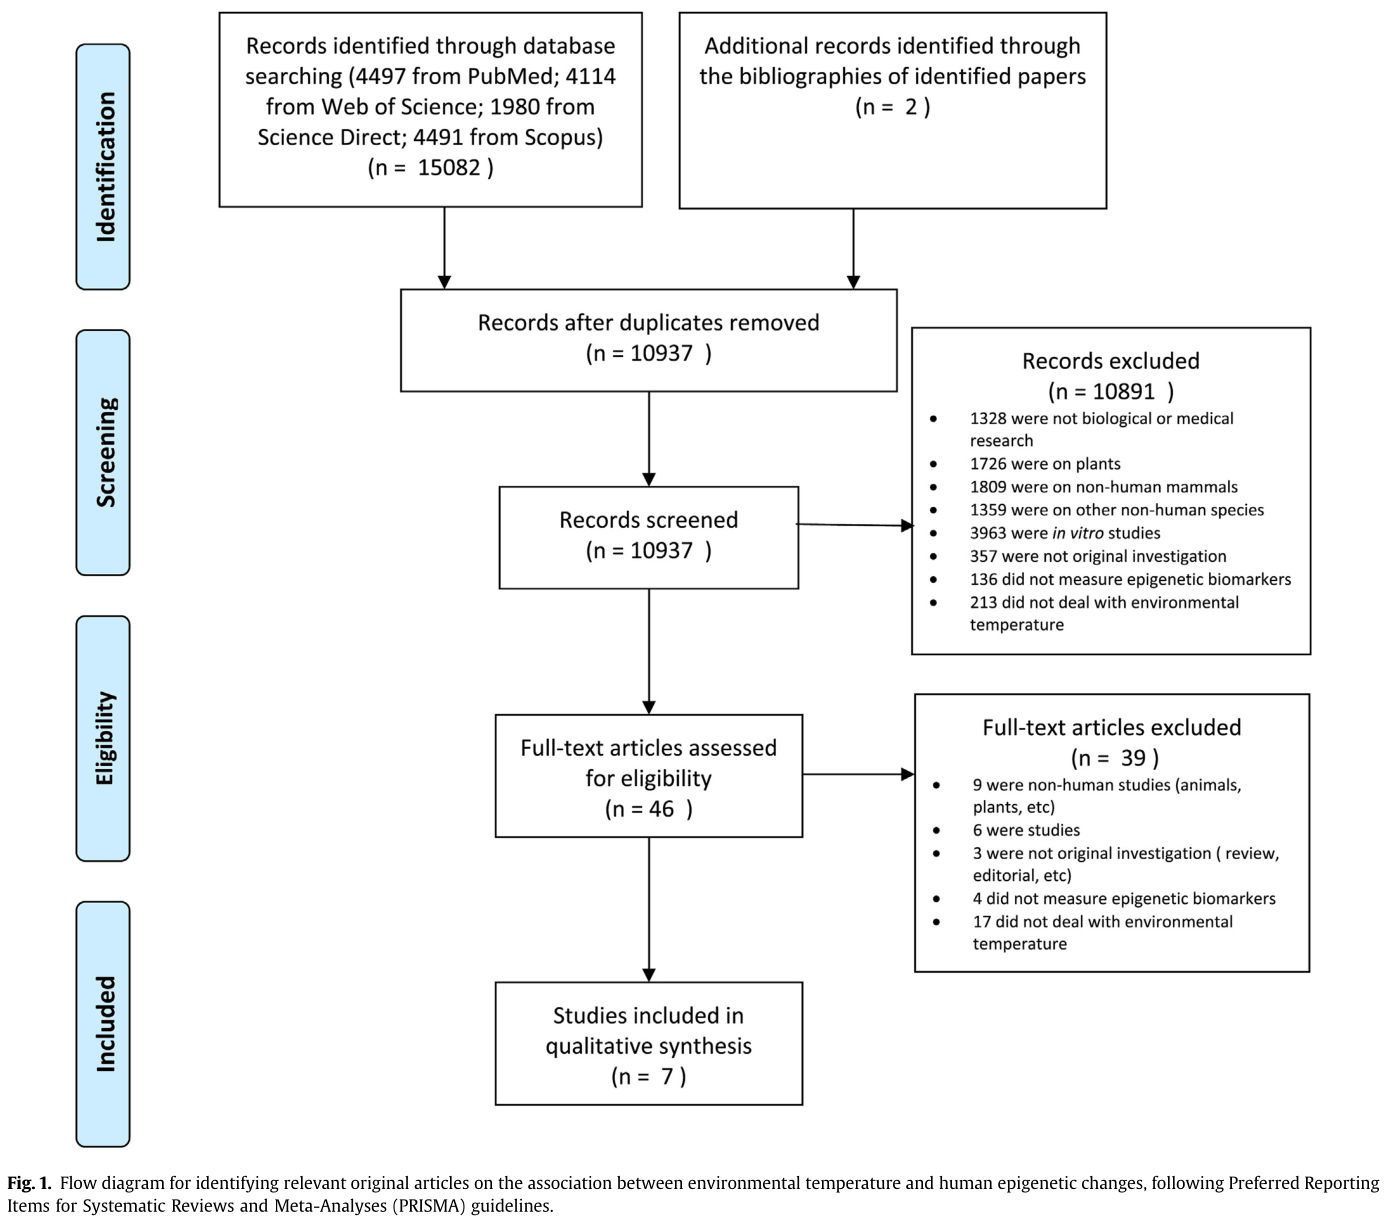
\includegraphics[scale=0.33]{images/fig-4-1.png} % chktex-8
  \end{figure}
\end{itemize}

\subsection{Results}
\begin{itemize}
  \item Short-term ambient temperature could affect global DNA
  methylation;
  \item A total of 15 candidate genes (ICAM-1, CRAT, F3, TLR-2, iNOS,
  ZKSCAN4, ZNF227, ZNF595, ZNF597, ZNF668, CACNA1H, AIRE, MYEOV2, NKX1-2 and CCDC15) with methylation status associated with short-term ambient temperature have been identified;
  \item DNA methylation on ZKSCAN4, ICAM-1 partly mediated the effect of short-term cold temperature on high blood pressure and ICAM-1 protein (related to cardiovascular events), respectively;
  \item Short-term ambient temperature might affect the human’s
  proportions of leukocyte subtypes estimated by Illumina 450 k
  data in blood sample.
\end{itemize}

\subsection{Discussion}
\begin{itemize}
    \item Many questions remained unanswered and limited data of this study provided little conclusive findings, so the authors of this paper created a mind map with various hierarchical subject ares of interest that should be investigated to better understand the link between epigenetic modifications and environmental temperature exposure.
      \begin{itemize}
        \item \textbf{Epigenetic modifications}:
          \begin{itemize}
            \item Multi-omics integration; other epigenetic regulation factors could be at play.
            \item Further study of DNA methylation; cost, number of studies, and limited data provide little data to connect the multidimensional aspect of many of the modifications.
            \item Tissue specific epigenetic profiles; most studies rely on easily accessible tissue, but DNA methylation can work differently cross-tissue, especially early in development. 
          \end{itemize}
        \item \textbf{Environmental temperature}:
          \begin{itemize}
            \item Exposure assessment; many studies did not focus on temperate, it was merely a covariant, so many were not measured on an individual level.
            \item Time windows; many studies focused on short term effects, long term effects of sub-optimal temperature exposure needs to be measured.
            \item Exposure level; many studies only related to low temperatures, there little data examining range of temperatures (and warmer).
            \item Other environmental factors; temperature could play a small role, air pollution, humidity, green space, socioeconomic status, and more may affect epigenetic responses to temperature.
          \end{itemize}
        \item \textbf{Methodological issues}:
          \begin{itemize}
            \item Study design; all studies were observational, both twin studies, randomized controlled trials could be helpful, but are costly.
            \item Study population; studies focused on young and elderly, which may be more vulnerable to temperature exposure, research is needed on general population samples.
            \item Statistical methods; many Bayesian and machine learning models could be applied to the data rather than just linear regressions. 
          \end{itemize}
      \end{itemize}
\end{itemize}

\end{itemize}

\nocite{xu2020environmental}
\bibliographystyle{apacite}
\bibliography{summaries.bib}
\end{document}